\noindent\markforreview
\vspace{1em}

For the function $f$, for each increase in the value of $x$ by $c$, where $c$ is a positive constant, the value of $f(x)$ increases by a factor of $27$. Which of the following equivalent forms of the function $f$ displays $\frac{1}{c}$ as a coefficient of $x$?

\vspace{0.75em}

\choicebox{A}{$f(x) = 54(3)^{\frac{1}{3}x}$}
\choicebox{B}{$f(x) = 54(3^3)^{\frac{1}{6}x}$}
\choicebox{C}{$f(x) = 54(9)^{\frac{1}{4}x}$}
\choicebox{D}{$f(x) = 54\left(27^{\frac{1}{3}x} \right)^{\frac{1}{2}}$}

\vspace{2em}
\newpage

\noindent\markforreview
\vspace{1em}

The composition of an animal is defined as the muscles, bones, and fat of the animal. A scientist studied the composition of one young swamp buffalo and determined the buffalo had $133$ kilograms of muscle, which made up approximately $65.9\%$ of its composition. Of the remaining composition of this buffalo, approximately $46.2\%$ was bone, and the remainder was fat. Based on these approximations, to the nearest tenth, how many kilograms of this buffalo's composition was bone?

\vspace{2em}
\newpage

\noindent\markforreview
\vspace{1em}

\[f(x) = 3(x-a)(x-b)(x-c)\]


The function $f$ is defined by the given equation, where $a$, $b$, and $c$ are distinct constants. When $a < x < b$, the value of $f(x)$ is positive. The graph of $y = f(x)$ in the $xy$-plane contains the point $(r, s)$, where $r$ and $s$ are constants. If $s = 8$, which of the following could be true?

\begin{itemize}
\item[I.] $r < a$
\item[II.] $b < r < c$
\item[III.] $r > c$
\end{itemize}

\vspace{0.75em}

\choicebox{A}{I only}
\choicebox{B}{III only}
\choicebox{C}{I and III only}
\choicebox{D}{II and III only}

\vspace{2em}
\newpage

\noindent\markforreview
\vspace{1em}

In isosceles triangle $ABC$, sides $AB$ and $AC$ are congruent. Point $D$ divides side $BC$ such that the length of $\overline{BD}$ is $\dfrac{4}{7}$ of the length of $\overline{BC}$. Point $E$ lies on side $AB$ and point $F$ lies on side $AC$ such that when segments $\overline{DE}$ and $\overline{DF}$ are drawn, angle $\angle BED$ is congruent to angle $\angle CFD$. If the length of $\overline{BE}$ is $8$, what is the length of $\overline{CF}$?

\vspace{0.75em}

\choicebox{A}{6}
\choicebox{B}{14}
\choicebox{C}{32}
\choicebox{D}{56}

\vspace{2em}
\newpage

\noindent\markforreview
\vspace{1em}

The function $f$ is defined by the given equation: 
\[
f(x) = x^2 - 4x - 320
\]
Which of the following equivalent forms of the equation displays the minimum value of the function as a constant or coefficient?

\vspace{0.75em}

\choicebox{A}{$f(x) = x^2 - 4(x + 80)$}
\choicebox{B}{$f(x) = (x - 2)^2 + (-324)$}
\choicebox{C}{$f(x) = x(x - 4) + (-320)$}
\choicebox{D}{$f(x) = (x + 16)(x - 20)$}

\vspace{2em}
\newpage

\noindent\markforreview
\vspace{1em}

In the given equation, $s$ and $r$ are constants, and $s > 0$. If the equation has infinitely many solutions, what is the value of $s$?
\[
\frac{12x + 28}{4} - \frac{s}{13} = r(x - 8)
\]

\vspace{2em}
\newpage

\noindent\markforreview
\vspace{1em}

The function $f$ is defined by $f(x) = -39^x$. The function $g$ is a decreasing linear function.  
In the $xy$-plane, the graphs of $y = f(x)$ and $y = g(x)$ intersect at two points, $(h, j)$ and $(k, m)$, where $j > m$.  
When $g(x) < f(x)$, which of the following must also be true?

\vspace{0.75em}

\choicebox{A}{$x > k$}
\choicebox{B}{$x < h$}
\choicebox{C}{$x > k$ or $x < h$}
\choicebox{D}{$h < x < k$}

\vspace{2em}
\newpage

\noindent\markforreview
\vspace{1em}

A circle in the $xy$-plane has its center at $(-7, 3)$ and has a radius of $9$.  
An equation of this circle is $x^2 + y^2 + ax + by + c = 0$, where $a$, $b$, and $c$ are constants.  
What is the value of $c$?

\vspace{2em}
\newpage

\noindent\markforreview
\vspace{1em}

At different times on a certain day, a manager at a theme park recorded the number of visitors.  
An exponential model gives the estimated number of visitors, $V$, at the theme park $t$ hours after the theme park opened, where $t \leq 3$.  
Based on the model, 80 visitors were estimated to be at the theme park when it opened,  
and every 30 minutes the estimated number of visitors increased by 150\% of the number 30 minutes earlier.  
Which of the following equations best represents this model?

\vspace{0.75em}

\choicebox{A}{$V = 80(2.5)^{2t}$}
\choicebox{B}{$V = 80(2.5)^{\frac{t}{30}}$}
\choicebox{C}{$V = 80(1.5)^{2t}$}
\choicebox{D}{$V = 80(1.5)^{\frac{t}{30}}$}

\vspace{2em}
\newpage

\noindent\markforreview
\vspace{1em}

The function $m$ gives the predicted body mass $m(t)$, in kilograms (kg), of a male giraffe $t$ days after it was born in a wildlife reserve, where $t \leq 390$.  
\[
m(t) = -0.0274\left(\frac{t}{7}\right)^2 + 7.3873\left(\frac{t}{7}\right) + 75.032
\]  
Which of the following is the best interpretation of the statement “$m(370)$ is approximately equal to $389$” in this context?

\vspace{0.75em}

\choicebox{A}{The predicted body mass of a male giraffe was approximately 370 kg 389 days after it was born.}
\choicebox{B}{The predicted body mass of a male giraffe was approximately 389 kg 370 days after it was born.}
\choicebox{C}{The predicted body mass of a male giraffe was approximately 389 kg $\frac{370}{7}$ days after it was born.}
\choicebox{D}{The predicted body mass of a male giraffe was approximately $\frac{370}{7}$ kg 389 days after it was born.}

\vspace{2em}
\newpage

\noindent\markforreview
\vspace{1em}

At a hotel, guests used the pool for a total of $t$ hours in March. At the same hotel, guests used the pool for $3.61t$ hours in April.  
What is the percent increase in the number of hours guests used the pool from March to April?

\vspace{0.75em}

\choicebox{A}{$2.61\%$}
\choicebox{B}{$3.61\%$}
\choicebox{C}{$261\%$}
\choicebox{D}{$361\%$}

\vspace{2em}
\newpage

\noindent\markforreview
\vspace{1em}

For data set A, the table summarizes the distribution of the number of pieces of mail received by a business each day during a period of 11 days.

\[
\begin{array}{|c|c|}
\hline
\text{Pieces of mail} & \text{Days} \\
\hline
0 & 2 \\
4 & 2 \\
5 & 2 \\
6 & 2 \\
7 & 1 \\
8 & 1 \\
17 & 1 \\
\hline
\end{array}
\]

The data value $17$ is removed from data set A to create data set B, which consists of the remaining 10 data values.  
Which statement best compares the median of data set A and the median of data set B?

\vspace{0.75em}

\choicebox{A}{The median of data set B is less than the median of data set A.}
\choicebox{B}{The median of data set B is greater than the median of data set A.}
\choicebox{C}{The median of data set B is equal to the median of data set A.}
\choicebox{D}{There is not enough information to compare the medians of the two data sets.}

\vspace{2em}
\newpage

\noindent\markforreview
\vspace{1em}

Triangle $ABC$ is similar to triangle $DEF$, where $A$ corresponds to $D$ and $C$ corresponds to $F$.  
Angles $C$ and $F$ are right angles.  
If $\tan(A) = \sqrt{5}$ and $DF = 53$, what is the length of $DE$?

\vspace{0.75em}

\choicebox{A}{$\dfrac{53\sqrt{3}}{5}$}
\choicebox{B}{$\dfrac{53\sqrt{3}}{2}$}
\choicebox{C}{$53\sqrt{6}$}
\choicebox{D}{$106$}

\vspace{2em}
\newpage

\noindent\markforreview
\vspace{1em}

A triangular pyramid has exactly six edges. Each of these edges is 96 centimeters long.  
If the surface area of the pyramid is $k\sqrt{3}$ square centimeters, what is the value of $k$?

\vspace{0.75em}

\choicebox{A}{2304}
\choicebox{B}{4608}
\choicebox{C}{6912}
\choicebox{D}{9216}

\vspace{2em}
\newpage

\noindent\markforreview
\vspace{1em}

For the positive quantities $h$, $j$, and $k$, 44\% of $h$ is equivalent to 62\% of $j$, and $j$ is equivalent to 22\% of $k$.  
What percentage of $k$ is $h$?  
(Disregard the \% sign when entering your answer. For example, if your answer is 39\%, enter 39)

\vspace{2em}
\newpage

\noindent\markforreview
\vspace{1em}

A right circular cone has a volume of $34{,}496\pi$ cubic centimeters and the area of its base is $3{,}136\pi$ square centimeters.  
What is the slant height, in centimeters, of this cone?

\vspace{0.75em}

\choicebox{A}{11}
\choicebox{B}{33}
\choicebox{C}{56}
\choicebox{D}{65}

\vspace{2em}
\newpage

\noindent\markforreview
\vspace{1em}

A quadratic function models the height, in feet, of an object above the ground in terms of the time, in seconds, after the object was launched.  
According to the model, the object was launched from a height of 0 feet and reached its maximum height of 400 feet 5 seconds after it was launched.  
Based on the model, what was the height, in feet, of the object 9 seconds after it was launched?

\vspace{2em}
\newpage

\noindent\markforreview
\vspace{1em}

An environmental scientist is investigating the volatility of 175 organic compounds by finding the boiling point of each compound.  
The mean boiling point of all 175 compounds is 167 degrees Celsius.  
The scientist classifies each of these compounds as either semivolatile or volatile.  
Of the 175 compounds, 50 compounds were classified as semivolatile, and these 50 compounds have a mean boiling point of 322 degrees Celsius.  
The remaining 125 compounds were classified as volatile.  
What is the mean boiling point, in degrees Celsius, of the 125 compounds classified as volatile compounds?

\vspace{2em}
\newpage

\noindent\markforreview
\vspace{1em}

A carpenter charges a flat rate of \$228 for the first 2 hours of work and \$95 for each additional hour of work.  
Which equation gives the total amount $y$, in dollars, that the carpenter charges for $x$ hours of work, where $x > 2$?

\vspace{0.75em}

\choicebox{A}{$y = 95x + 228$}
\choicebox{B}{$y = 228x + 418$}
\choicebox{C}{$y = 95x + 38$}
\choicebox{D}{$y = 228x + 95$}

\vspace{2em}
\newpage

\noindent\markforreview
\vspace{1em}

On a plot of land, 48.0\% of the square footage is farmland and the remaining square footage is pasture.  
There are buildings on exactly 23.5\% of the square footage of the farmland, and there are buildings on exactly 16.0\% of the square footage of the pasture.  
If there are buildings on exactly $p\%$ of the square footage of the plot of land, what is the value of $p$?

\vspace{2em}
\newpage

\noindent\markforreview
\vspace{1em}

A company developed a plan to set the selling price of a product.  
The company determined that for a selling price of \$120.00, zero products would be sold.  
For each \$2.50 decrease in the selling price, the number of products sold would increase by one.  
For a revenue of exactly \$1,437.50, which of the following could be the number of products sold?  
(revenue = price $\times$ number of products sold)

\vspace{0.75em}

\choicebox{A}{23}
\choicebox{B}{24}
\choicebox{C}{527}
\choicebox{D}{1,440}

\vspace{2em}
\newpage

\noindent\markforreview
\vspace{1em}

A circle in the $xy$-plane has its center at $(2, 9)$.  
Line $t$ is tangent to this circle at the point $(a, -4)$, where $a$ is a constant.  
The slope of line $t$ is $\frac{6}{5}$.  
What is the value of $a$?

\vspace{0.75em}

\choicebox{A}{$-\frac{68}{5}$}
\choicebox{B}{$-\frac{53}{6}$}
\choicebox{C}{$\frac{77}{6}$}
\choicebox{D}{$\frac{88}{5}$}

\vspace{2em}
\newpage

\noindent\markforreview
\vspace{1em}

\begin{center}
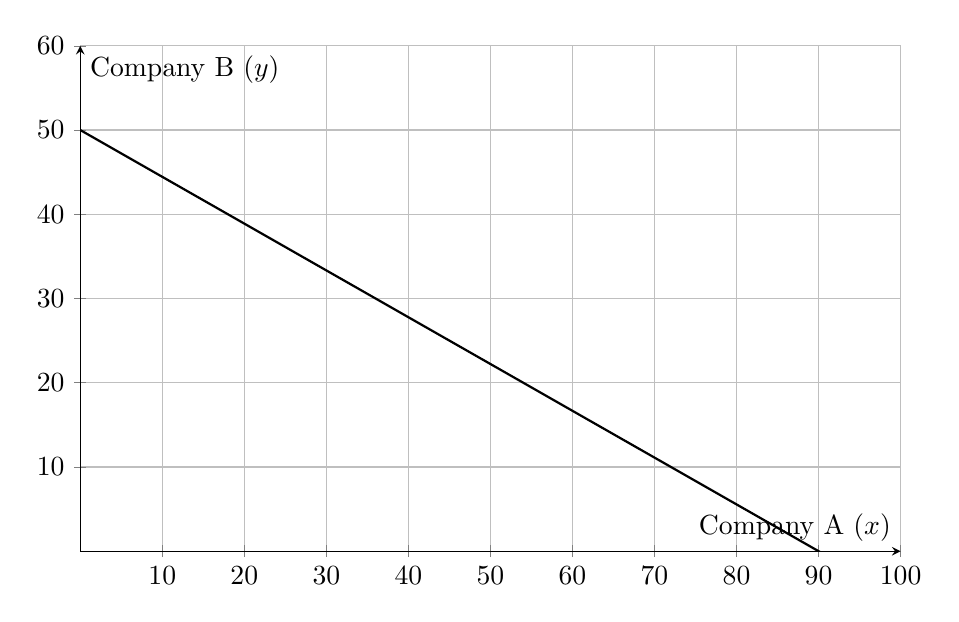
\begin{tikzpicture}
\begin{axis}[
    axis lines = middle,
    xlabel = {Company A ($x$)},
    ylabel = {Company B ($y$)},
    xmin=0, xmax=100,
    ymin=0, ymax=60,
    grid = both,
    width=12cm,
    height=8cm,
    samples=100,
    domain=0:100,
    legend pos=north east,
]
\addplot[
    thick,
    black,
]
{(900 - 10*x)/18};
\end{axis}
\end{tikzpicture}
\end{center}

The graph shows the relationship between the number of shares of stock from Company A, $x$,  
and the number of shares of stock from Company B, $y$, that Sayen can purchase.  
Which equation could represent this relationship?

\vspace{0.75em}

\choicebox{A}{$y = 10x + 18$}
\choicebox{B}{$10x + 18y = 900$}
\choicebox{C}{$y = 18x + 10$}
\choicebox{D}{$18x + 10y = 900$}

\vspace{2em}
\newpage

\noindent\markforreview
\vspace{1em}

The scatterplot shows data set $A$, which consists of the weights $y$, in pounds,  
of a Labrador retriever puppy at various ages, $x$, in months.  
The equation of a line of best fit for the relationship in data set $A$ can be written as  
$y = -5.1 + 8.7x$, where $2 \leq x \leq 6$.





\begin{center}
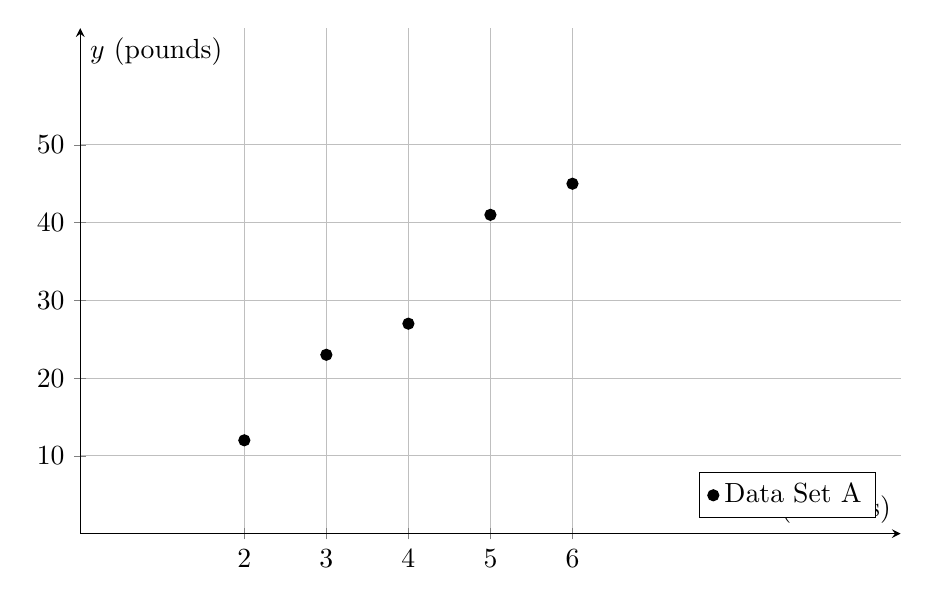
\begin{tikzpicture}
\begin{axis}[
    axis lines=middle,
    xlabel={$x$ (months)},
    ylabel={$y$ (pounds)},
    xmin=0, xmax=10,
    ymin=0, ymax=65,
    xtick={0,2,3,4,5,6},
    ytick={0,10,20,30,40,50},
    grid=both,
    legend pos=south east,
    width=12cm,
    height=8cm
]





% Original data points
\addplot[
    only marks,
    mark=*,
    mark size=2pt
]
coordinates {
    (2, 12)
    (3, 23)
    (4, 27)
    (5, 41)
    (6, 45)
};
\addlegendentry{Data Set A}

;

\end{axis}
\end{tikzpicture}
\end{center}




The puppy was weighed again at 9 months old and weighed 52 pounds.  
Data set $B$ consists of all the data points in data set $A$ as well as the data point $(9, 52)$.  
The equation of a line of best fit for data set $B$ can be written as $y = r + sx$,  
where $r$ and $s$ are constants and $2 \leq x \leq 9$.  
Assuming the equations of the lines of best fit are calculated in the same way,  
which of the following is the best estimate for the value of $s$?

\vspace{0.75em}

\choicebox{A}{5.9}
\choicebox{B}{8.7}
\choicebox{C}{13.8}
\choicebox{D}{17.7}

\vspace{2em}
\newpage

\noindent\markforreview
\vspace{1em}

In the given equation, $b$ is an integer. The equation has no real solutions.  
What is the least possible value of $b$?

\[
-x^2 + bx - 49 = 0
\]

\vspace{2em}
\newpage

\noindent\markforreview
\vspace{1em}

For a study, a group of gophers will be selected from a habitat consisting of 220 gophers, and a group of groundhogs will be selected from a habitat consisting of 200 groundhogs. Some of the gophers and groundhogs will be in a treatment group, and some of the gophers and groundhogs will be in a control group. Which of the following is necessary for this study to attempt to establish a cause-and-effect relationship between two variables?

\vspace{0.75em}

\choicebox{A}{The number of gophers in the treatment group is equal to the number of groundhogs in the treatment group, and the number of gophers in the control group is equal to the number of groundhogs in the control group.}
\choicebox{B}{The gophers and the groundhogs are randomly selected from their respective habitats.}
\choicebox{C}{The gophers and the groundhogs are randomly assigned to the treatment and control groups.}
\choicebox{D}{The average age of the gophers in the treatment group is equal to the average age of the groundhogs in the treatment group, and the average age of the gophers in the control group is equal to the average age of the groundhogs in the control group.}

\vspace{2em}
\newpage
